% igs2eguide.tex
% v2.00 12-jun-08

\NeedsTeXFormat{LaTeX2e}

% The default is for Journal of Glaciology, one column, A4 paper. The other options are listed below:

%\documentclass{igs}
%   \documentclass[twocolumn]{igs}
% \documentclass[annals]{igs}
% \documentclass[annals,twocolumn]{igs}

% \documentclass[letterpaper]{igs}
% \documentclass[twocolumn,letterpaper]{igs}
% \documentclass[annals,letterpaper]{igs}
% \documentclass[annals,twocolumn,letterpaper]{igs}

% when submitting your article for review, use one
% of the following two options:

\documentclass[review]{igs}
% \documentclass[annals,review]{igs}

  \usepackage{igsnatbib}
  \usepackage{stfloats}

% check if we are compiling under latex or pdflatex
  \ifx\pdftexversion\undefined
    \usepackage[dvips]{graphicx}
  \else
    \usepackage[pdftex]{graphicx}
  \fi

\usepackage[T1]{fontenc}
\usepackage{lmodern} %this is needed with T1
\usepackage[utf8]{inputenc}  


%\pdfcompresslevel=9 

% the default is for unnumbered section heads
% if you really must have numbered sections, remove
% the % from the beginning of the following command
% and insert the level of sections you wish to be
% numbered (up to 4):

% \setcounter{secnumdepth}{2}

\begin{document}

\title[Glacier observations using TRI]{Multi-year observations of Brei{\dh}amerkurjökull, a marine-terminating glacier in southeastern Iceland, using Terrestrial Radar Interferometry}

\author[Voytenko and others]{Denis VOYTENKO$^1$, Timothy H. DIXON$^1$,
  Ian M. HOWAT$^2$, Noel GOURMELEN$^3$, Chad LEMBKE$^4$, Charles L. WERNER$^5$, Santiago de la PEÑA$^2$,   Björn ODDSSON$^6$}

\affiliation{%
$^1$School of Geosciences,
University of South Florida, Tampa, Florida, USA.\\
E-mail: dvoytenk@mail.usf.edu\\
$^2$School of Earth Sciences and Byrd Polar Research Center, The Ohio State University,
Columbus, Ohio, USA.\\
$^3$School of Geosciences, University of Edinburgh, Edinburgh, United Kingdom.
$^4$College of Marine Science, University of South Florida, St. Petersburg, Florida, USA.
$^5$Gamma Remote Sensing, Gümligen, Switzerland.
$^6$Feltfélagið, Kopavógur, Iceland.}


\abstract{Terrestrial Radar Interferometry (TRI) is a new technique for studying ice motion and volume change of glaciers. TRI is especially useful for temporally and spatially-dense measurements of highly dynamic glacial termini. We conducted a TRI survey of Brei{\dh}amerkurjökull, a marine-terminating glacier in Iceland, imaging its terminus near the end of the melt season in 2011, 2012, and 2013. The ice velocities were as high as 5 m/d, with the fastest velocities near the calving front. Measurement uncertainties are approximately 0.05 m/d. Retreat of the glacier over the three year observation period was accompanied by strong embayment formation. Iceberg tracking with the radar shows high current velocities near the embayment, probably indicating strong meltwater outflow and mixing with relatively warm lagoon water.}
%add (3$^{\circ}$C)
\maketitle



\section{Introduction}
Melting of the ice sheets covering Greenland and Antarctica is accelerating, presumably in response to rising global temperatures \citep{wouters2008grace, jiang2010accelerating, rignot2011acceleration, shepherd2012reconciled}. Ocean forcing, where warm, saline (hence dense) water undercuts the deeper parts of marine-terminating glaciers \citep{motyka2003submarine} is believed to be an important aspect of accelerating ice loss on both continents \citep{payne2004recent,shepherd2004warm,holland2008acceleration,straneo2010rapid,straneo2012characteristics,joughin2012ice,park2013sustained}. However, studying this process is challenging, as it involves measurements in or near the highly dynamic ice-ocean interface.
  

Brei{\dh}amerkurjökull is a large outlet glacier for Vatnajökull, Iceland’s main ice cap (Figure \ref{fig:sitelocation}). Aerial photography presented by \citet{bjornsson2001jokulsarlon} suggests that the glacier has been retreating for most of the 20th century. The glacier has a mostly grounded ice front which calves into a 20 km$^2$ tidal lagoon (Jökulsárlón) on the south side of the island, making it an excellent “natural laboratory” for studying ice-ocean interactions \citep{howat2008dynamic}.  The lagoon has a maximum depth of 300 m and is connected to the North Atlantic Ocean through a 100-m wide by 20-m deep engineered channel lined with rip-rap \citep{bjornsson1996scales}. 

In 2011, 2012, and 2013, we deployed a Terrestrial Radar Interferometer (TRI) at Brei{\dh}amerkurjökull with four primary objectives: 1) to assess instrument performance; 2) to observe the influence of calving and tides on the instantaneous ice velocity; 3) to observe changes in ice mass, distribution, and retreat from year to year; 4) to assess the role of ocean currents in ice mass loss. The TRI is a newly developed technology with the potential to complement existing instrumentation for ice velocity measurements \citep{riesen2011short}. 
In contrast to point measurements provided by GPS receivers, the TRI provides a spatially continuous velocity field over 10's of km in extent and provides better temporal resolution (several minutes) compared to satellites, which have typical revisit times of several days or longer \citep{covello2010cosmo,werninghaus2010terrasar}, without the need for dangerous and/or expensive in situ deployments on unstable glacier surfaces. TRI also provides high-quality DEMs to determine surface slopes and ice volume change, and can be used in an iceberg tracking mode to infer surface currents. 
%We can also observe crevasse spacing and propagation with the TRI imagery.
% Thus, the TRI is an ideal instrument for observing ice velocity at high temporal and spatial resolution over glacier termini.
% Here we test the suitablity of TRI for a variety of glacier kinematic and dynamic studies.



\section{Methods}
\subsection{Instrument Description}
The TRI used for this study is the GAMMA Portable Radar Interferometer (GPRI). The GPRI is an interferometric, Ku-band (1.74 cm wavelength), real-aperture radar that provides high resolution intensity images and is also sensitive to line-of-sight surface displacements on the order of 1 mm \citep{werner2008real}. Two-dimensional velocities can potentially be determined with feature tracking. 
% Given the short radar wavelength, the signal scatters off the ice surface with minimal penetration. 
The range resolution of the GPRI is 0.75 m, independent of distance to a first approximation. The azimuth resolution of the GPRI at 1 km is 7.5 m, and scales linearly with distance. The radar has one transmitting antenna and two receiving antennas with a 25 cm baseline, and is positioned on a rotating frame (Figure \ref{fig:fieldsetup}). The radar takes approximately 90 seconds to scan and prepare data from a 100-degree arc. Consecutive interferograms from one transmitting-receiving antenna pair are used to observe the 
velocity. The presence of two receiving antennas allows mapping of the glacial topography to a 
vertical precision of about 3 m at 2 km distance \citep{strozzi2012topography}. 


\subsection{Data Collection and Analysis}
We imaged the glacier with the TRI for a number of multi-hour periods over 3 days in September of 2011, 4.5 days in August of 2012, and 2 days in August of 2013. Each year, we positioned the radar on moraine deposits  4 km away from the terminus in approximately the same spot. The location was easily accessible and provided a high vantage point to minimize interference from moving icebergs while being close enough to the terminus to minimize atmospheric noise. 


The radar scanned 50$^{\circ}$ arcs with a range of 2-6.5 km in 2011, 90$^{\circ}$ arcs with a range of 50 m to 8.5 km in 2012, and 100$^{\circ}$ arcs with a range of 50 m to 16.9 km in 2013. Velocity maps were constructed using 3.5-hour periods of 1-minute interferograms from 2011, and 3.5-hour periods of 3-minute interferograms from 2012 and 2013.


Radar image processing was done with the GAMMA software. The resulting imagery was converted into rectangular (map) coordinates with 10-meter pixel spacing. 
%The imagery used for year-to-year comparisons was also corrected for small rotation offsets around the the pixel containing the location of the radar. 
The TRI imagery was georeferenced by rotating the map coordinate data around the pixel containing the radar to produce the best visual match to a LANDSAT image.

Since the radar obtains high-precision displacement measurements via phase comparisons that are inherently ambiguous, the phase data must first be ``unwrapped'' to investigate changes. Phase differences between successive images were unwrapped using a minimum-cost-flow algorithm \citep{costantini1998novel}, and then converted into velocities. The radar images were multi-looked (averaged) in range by a factor of 10 to reduce noise.
% After the processing, negative values indicate motion away from the radar.

Phase-unwrapped images were converted into line-of-sight velocity maps using the equation:
  \begin{equation}v=\frac{-\lambda\phi}{4\pi\Delta t}\end{equation}  
where $v$ is velocity, $\lambda$ is radar wavelength, $\phi$ is unwrapped phase, and $\Delta t$ is the time difference between the acquisitions in the interferogram. Multiple velocity images were then stacked (averaged) to produce a representative velocity map for a given observation period. 

If the direction of ice motion and the surface slope are known, the measured line-of-sight velocities can be converted to ice velocities in the direction of motion by 
  \begin{equation} V_{glac}=\frac{V_{los}}{cos(\alpha)cos(\phi)sin(\theta)-cos(\theta)sin(\alpha)}\end{equation} 
Here, $V_{glac}$ is the velocity of the glacier in the direction of motion, $V_{los}$ is the measured velocity in the line-of-sight of the instrument, $\alpha$ is the surface slope, $\theta$ is the radar look angle, and $\phi$ is the offset angle in the horizontal plane between the direction of ice motion and the orientation of the radar \citep{kwokandfahnestock}.

We can simplify the above formula to obtain an approximation of the ice velocity in the direction motion by assuming zero surface slope ($\alpha=0$) and a horizontal look angle ($\theta=90$), reducing equation 2 to 
  \begin{equation}  V_{glac}=\frac{V_{los}}{cos(\phi)}\end{equation} 
 
 
We also compared the TRI velocity maps to TerraSAR-X velocity maps from about the same time period as our field campaigns. Preliminary TRI
velocity results and comparisons to TerraSAR-X from the 2011 deployment were presented in \citet{voytenko2012monitoring}.
We compared the TRI velocities with velocities derived from TerraSAR-X offset tracking by scaling both measurements to account for the direction of ice motion (140$^{\circ}$ clockwise from north) using equation 3 (Figure \ref{fig:velmaps}). Note that for the TRI the offset angle ($\phi$) varies between each scan line direction and the direction of ice motion. The TerraSAR-X velocities are based on 11-day offset tracking maps (Sep. 22 - Oct. 3, 2011; Aug. 17 - Aug. 28, 2012; Aug. 15 - Aug. 26, 2013) from track T147 processed using the method of \citet{strozzi2002glacier} and \citet{ paul2013glaciers}. We show the differences between the TerraSAR-X and TRI velocities in Figure \ref{fig:velmapserror}.

  
To investigate possible temporal variations in ice velocity with the TRI, we generated total displacement time series by adding up all of the successive phase difference measurements (converted to displacements) at a given pixel (Figures \ref{fig:12tslocs}-\ref{fig:nzts12}). Missing data in the time series were filled with the average displacement before the integration to smooth data gaps. The displacement time series represent velocity changes as slope changes.

We also looked at the variability in measured displacement of pixels of stationary targets to define atmospheric and instrument-related uncertainties in the velocity estimates and to define optimum averaging times (Figure \ref{fig:12error}). This is discussed in more detail in the results section.


% \subsection{DEM Generation}
We operated a continous tide gauge in 2011 to investigate the impact of the tidal cycle on glacial velocity (Figure \ref{fig:11tidedisp}). Unfortunately, in 2012, the tide gauge failed shortly after deployment. 


We constructed a series of Digital Elevation Models (DEMs) by stacking two hours of acquisitions unwrapped using an adaptive filtering algorithm \citep{goldstein1998radar} and converting unwrapped phase into elevation using a reference elevation point and assuming a horizontally-stationed radar \citep{strozzi2012topography}:
  
\begin{equation}z=\frac{\lambda}{2\pi}\frac{R}{B}\phi+\frac{B}{2}-\left(\frac{\lambda}{2\pi}\right)^2 \frac{\phi^2}{2B}\end{equation}
 
where $\lambda$ is the radar wavelength, $\phi$ is the unwrapped phase value (from an interferogram between the two receiving antennas at a given pixel), $B$ is the baseline (vertical offset between the two receiving antennas, 25 cm), and $R$ is the range distance from the radar to the given pixel. We masked out the lagoon and shadowed areas, and smoothed the DEM surface with a median filter. 


Using the method proposed by \citet{etzelmuller1993mass}, the DEMs are discretized into $N$ cells with edge length $d$ (10 m) and height $H$ ($H_{2011}$ and $H_{2012}$). The total ice volume change for the imaged area is
  
\begin{equation}\Delta V=\sum\limits_{i=1}^N d^2 \times (H_{2011}-H_{2012})_i\end{equation} where $i$ represents an individual cell in the DEM. DEMs for 2011 and 2012 and the change in ice volume are shown in Figures \ref{fig:demperspective} and \ref{fig:dems} respectively.
 
Assuming a constant ice density, $\rho_{ice}$, of 917 kg/m$^3$, and a constant water density, $\rho_{w}$, of 1000 kg/m$^3$, the total mass balance (MB) for the imaged area of the glacier ($A$) can be represented as the change in ice thickness in meters water equivalent (m w.e.) by
  
\begin{equation}MB=\frac{\rho_{ice}}{\rho_w} \times \frac{\Delta V}{A}\end{equation}
 

% \subsection{Salinity and Temperature Data Analysis}
In 2012 and 2013, the salinity and temperature of water in the lagoon were measured with a series of profiles, in order to assess the role of warm ocean water in glacier mass balance. 

In 2012, temperature and salinity data in the lagoon were collected with a bottom stationed ocean profiler (BSOP) \citep{langebrake2002design}. The BSOP is an autonomous buoy originally designed to profile the water column in the shelf margins of the Gulf of Mexico. Preliminary results were presented in \citet{DIXONEOS}. In 2013, we collected profiles of temperature and salinity in the lagoon by manual casts of a CTD (conductivity-temperature-depth) profiler from a small boat.
% For this study, the BSOP measured salinity and temperature as a function of depth in order to describe the stratification in Jökulsárlón.
The ascending and descending data from 2013 were averaged together over 1-meter intervals. Conductivity was converted to salinity using the method described by \citet{fofonoff1983algorithms}.  Given the relatively shallow depths (less than 200 meters), temperature was not converted to potential temperature.  The location of the profiles vary from day to day and year to year due to strong currents and iceberg cover.  However, most of the lagoon appears to be well-mixed (see Results below), hence the spatially-limited available data are believed to be representative. 
%In 2011 and 2013, data were collected by manual casts from a small boat.  In 2012 we tested an automated profiler, as described in \citet{DIXONEOS}. 


\section{Results}
\subsection{Terminus Position and Glacier Motion}
The terminus of the glacier shows a retreat rate on the order of 100 m/yr for the three year period 2011-2013, with the exception of the formation of seasonal, narrow, localized, embayment which retreats \textasciitilde500-700~m (Figure \ref{fig:retreat}) during the melt season, and partially closes during the winter months. 



% In each of the three observation years, the maximum line-of-sight velocities occur near the calving front, and are 3-5 m/d.
 Figure \ref{fig:velmaps} shows the average velocity measured with the TRI in a 3.5-hour period in the three observation years along with a comparison to 11-day TerraSAR-X velocity maps acquired around the same time period. 
%  The TRI and TerraSAR-X velocity maps have been adjusted to account for the direction of ice motion, 140$^{\circ}$. 
In each of the three observation years, the maximum velocities measured with the TRI occur near the calving front, and are 3-5$\pm$0.05 m/d. The velocity maps show that the zones of high velocity are located in a concentrated area near the calving front, with 2012 having a wider areal distribution of high velocities than 2011 and 2013. 




 Difference maps between the TerraSAR-X and TRI velocities are shown in Figure \ref{fig:velmapserror}. The comparisons are only done for the overlapping regions. Given the different averaging times between the TRI and TerraSAR-X (3.5 hours vs 11 days), the rms differences between the two instruments are relatively high: 0.8 m/d in 2011, 1 m/d in 2012, and 1 m/d in 2013, with the largest differences near the dynamic terminal zone. The short averaging time of the TRI may be capturing short-lived dynamic phenomena that are smoothed in the longer time-averaged satellite data. Differences between the two data sets are much smaller away from this dynamic zone.
% Both, TRI and TerraSAR-X velocityThe TerraSAR-X velocity maps are from track T147, and show projected horizontal motion onto the direction of ice motion, 140$^{\circ}$.
\citet{nagler2012retrieval} derived three-dimensional velocity fields from Brei{\dh}amerkurjökull in the fall of 2010 using TerraSAR-X, COSMO-SkyMed, and GPS data. Their results show that the glacier is moving southeast with average velocities of under 2 m/d a short distance away from the fast-moving terminus. This slower zone of motion is visible in both the TRI and TerraSAR-X data (Figure \ref{fig:velmaps}).


In 2011, when limited overlapping tide gauge and TRI data are available, there is no apparent relationship between tides and ice velocities in the short time series (Figure \ref{fig:11tidedisp}). This may reflect the mostly-grounded nature of the terminus, where minor changes in water depth have a negligible influence on the weight of the glacier, but longer time series are necessary for a thorough analysis.

%However, a longer continous radar time series would have been beneficial for a more detailed comparison. 

\subsection{Velocity Uncertainties}
We can calculate the velocity bias due to the zero surface slope assumption (equation 3) by approximating the surface slope from our DEM data. As discussed in the next section (DEMs and Mass Change), the surface slope of the first 500~m at the terminus is \textasciitilde14$^\circ$ while the slope of ice immediately behind the first 500~m of the ice cliff is \textasciitilde2$^\circ$. The upglacier slopes can also be verified using elevation data presented by \citet{bjornsson2001jokulsarlon}. Using these slope values for $\alpha$ in equation 2 suggests that assuming a zero surface slope can lead to errors of around 3 percent over the first 500~m of the terminus, with errors much less than 1 percent further upglacier.

Results from the TRI are sensitive to water vapor in the atmosphere.  Water vapor attenuates and slows the microwave signal, decreasing signal to noise ratio and increasing the two way travel time between the instrument and target by variable amounts.  This impacts the phase measurements, and hence affects both the displacement time series and the DEM estimation.  A humid atmosphere can also degrade instrument performance.  For example, water droplets condensing on the antenna attenuate the transmitted and received signals and may also corrupt the phase of the received signal independent of atmospheric transmission effects.  

While it is highly variable in both space and time, on average, the amount of water vapor typically decreases rapidly with height in the troposphere.  Compared to satellite SAR, where the slant range signal path is typically within about 35$^{\circ}$ of vertical, the TRI signal transits through that portion of the atmosphere where water vapor concentrations tend to be highest.  Thus, water vapor can have a larger impact on ground-based TRI compared to satellite radar interferometers. Atmospheric moisture was typically high during our observations, as evidenced by persistent fog, clouds, and rain. For all these reasons, it is important to quantify the effects of water vapor on the TRI results.  We will show that while water vapor is almost certainly the largest source of noise for the TRI’s displacement time series and ice velocity estimates in our Iceland data set, its effects are nevertheless small compared to signals of interest for most glaciological investigations.  

Figure \ref{fig:ts12} shows displacement time series for several points on the glacier and marginal areas for one 24 hour period in 2012.   The slope of a best fit line through the phase-connected displacement estimates represents the average velocity over that period, and the rms scatter of the fit (1-21 mm) is one measure of displacement precision.   However, it is overly conservative, as some of the scatter represents real velocity variation of the glacier over the 24 hour observation period.  The rms scatter of the three points known to be stable (1-8 mm; Figure \ref{fig:nzts12}) is a better indicator of displacement precision. For these latter three points, the lowest rms scatter (1 mm) is observed for the closest point (4.2 km), while larger scatter (8 mm) is observed for points farther away (6.2 and 7.9 km), consistent with the influence of water vapor.  In dry air, the inherent precision of the TRI, observed over distances less than a kilometer, is a few tenths of a millimeter or less \citep{werner2008real}.  From the three 
nominally stable points adjacent to the glacier (Figure \ref{fig:12tslocs}), where we expect $v=0$, we can also estimate the total velocity error (water vapor plus other effects) by looking at deviation from zero, suggesting that velocity uncertainty is 0.05 m/d or less (Figure \ref{fig:nzts12}).

For many applications, it is desirable to investigate velocity variations for times much shorter than one day.  Since there is a trade-off between velocity uncertainty and averaging time for any displacement measurement technique, it is useful to quantify velocity uncertainty as a function of averaging time.   
The velocity or rate uncertainty ($\sigma_r$) based on a series of displacement measurements is a function of the displacement measurement precision (we assume $\sigma_m$=1~mm) and the total time span of observations, $T$.  Assuming equally spaced (1-minute) observations, $\Delta t$, and assuming that measurement noise is ``white'' (uncorrelated in time), rate uncertainty is given by \citep{coates1985space,dixon1991introduction,mao1999noise}: 

  
\begin{equation}\sigma_r=\frac{\sigma_m}{T}\Bigg[\frac{12T/\Delta t}{(1+T/\Delta t)(2+T/\Delta t)}\Bigg]^{\frac{1}{2}}\end{equation}
 

Figure \ref{fig:12error} shows how the rate uncertainty evolves for different averaging times assuming measurement noise of 1 and 8 mm.  It is apparent that for any averaging time greater than about one hour, the rate uncertainty becomes negligible, even for distant points where water vapor effects can be relatively high, assuming measurement noise is white.   Observations of velocity variations over shorter periods are not precluded, but some caution or specialized techniques may be required.  

Atmospheric noise is not purely white, and hence may not reduce with long averaging times.  One way to assess deviations from the white noise approximation is to compare the velocity variation over stationary points for different averaging times. We investigated this by imaging the stationary points and calculating the velocity error by obtaining the displacement from zero to every known point in time, and dividing by the time since the measurements were started. The results of this calculation are also shown in Figure \ref{fig:12error}.  These results suggest that even for inherently noisy points (distant points and a humid atmosphere) velocity errors less than 0.5 m/day can be obtained with averaging times of about one hour.

\subsection{DEMs and Mass Change}
% 
The DEMs and their difference are shown in Figures \ref{fig:demperspective} and \ref{fig:dems}. More ice is lost in the immediate vicinity of the calving front, especially near the area of a newly-formed embayment.  Figure \ref{fig:velelev} shows the relationship between the surface slope and velocity in 2011 and 2012 near the calving front (high slope equals high velocity).

% For isostatic calculations it is also useful to know the mass change.
% Further below we quote change in both meters water equivalent (m w.e.) and mass (Gt). 

% The overall ice loss rate for the overlapping imaged area is 9$\pm$2 m/yr water equivalent, or 0.08$\pm$0.02 Gt/yr. More ice is lost in the immediate vicinity of the calving front, especially near the area of a newly-formed embayment. 


To describe the measurement uncertainty associated with the TRI-derived DEM, we compared the 2012 TRI DEM with the ASTER GDEM by resampling the pixel spacing in the TRI DEM to 30 meters (The ASTER GDEM is a product of METI and NASA) and matching the two data sets.  The ASTER GDEM is a satellite-derived DEM with 30-meter pixel spacing and a vertical accuracy of 17 m with a 95\% confidence \citep{aster2011validation}.  

Since the orientation of the TRI imagery is visually georeferenced to a LANDSAT image from May 23, 2013 (obtained from http://landsatlook.usgs.gov/), we consider the spatial georeferencing error to be on the order of 1 pixel (30~m due to DEM spacing). As the TRI and ASTER DEMs were not obtained at the same time, we selected a stationary mountainous area in both images for our comparison (Figure \ref{fig:dems}). The rms vertical difference between the TRI DEM and the ASTER GDEM is approximately 16 m. The high relief of the study area is likely an important factor contributing to this difference (geolocation error). Given the 30-meter spatial 
resolution in the 
resampled product, a horizontal difference of even one half-pixel (15~m) may 
mean a large difference in elevation at steep mountainsides.


We performed a similar analysis to estimate the year-to-year error between the TRI DEM in 2011 and 2012. We selected a stationary area (Figure \ref{fig:dems}) over moraine deposits for the comparison. The rms difference in this area between the TRI DEM in 2011 and 2012 is on the order of 2 m, suggesting that this is the minimum error for the ice loss estimates.

The DEMs generated from each year’s observations allow a quantitative assessment of mass change in the overlapping imaged area. We describe two possible approaches with uncertainties based on the 2-meter TRI DEM difference:

1. A minimum estimate of mass change is based on differencing of the overlapping images from successive years (Figures \ref{fig:demperspective} and \ref{fig:dems}) and applying Equations 5 and 6. This suggests a mass loss of \textasciitilde0.08$\pm$0.02 Gt/yr (9$\pm$2~m w.e.). This is a minimum estimate because the overlapping data only account for pixels which have nonzero elevations over both years, and hence method misses the part of the margin that has receded between the first and second year (Figure \ref{fig:demperspective}). 

2.  If we know the thickness of ice in the terminal region, equivalent to knowing bedrock elevation or the depth of the lagoon in front of the grounded ice given our DEM, we can measure the area and height of ice that is missed in the first approach, \textasciitilde0.6 square kilometers with an average loss rate of about 15$\pm$2~m w.e. (this is the part of the terminus that fully retreated between 2011 and 2012), and add it to the mass change estimated in 1. Assuming a lagoon depth of 200~m (to one significant figure) from the bedrock topography data of \citet{bjornsson2001jokulsarlon} and Figure 1 suggests an extra 0.1$\pm$0.1 Gt/yr of loss, for a total mass loss rate of \textasciitilde0.2$\pm$0.1 Gt/yr (10$\pm$5~m w.e.).

We can also compare our ice loss rate estimate to ice loss from the larger region of Vatnajökull. Our minimum loss estimate of approximately 9$\pm$2 m w.e. falls within the overall summer balance rate (-9.5 to 2.5 m w.e.) suggested by \citet{bjornsson2008icelandic}.

% The overall ice loss rate for the overlapping imaged area is 9$\pm$2 m/yr water equivalent, or 0.08$\pm$0.02 Gt/yr. More ice is lost in the immediate vicinity of the calving front, especially near the area of a newly-formed embayment. 



% 
% The DEMs and their difference are shown in Figures \ref{fig:demperspective} and \ref{fig:dems}. For isostatic calculations it is also useful to know the mass change. Below we quote change in both meters water equivalent (m w.e.) and mass (Gt). The overall ice loss rate for the overlapping imaged area is 9$\pm$2 m/yr water equivalent, or 0.08$\pm$0.02 Gt/yr. More ice is lost in the immediate vicinity of the calving front, especially near the area of a newly-formed embayment. 


\subsection{Iceberg-Current Observations}
Visual tracking of iceberg motion using successive intensity images can be used as a proxy for surface and near-surface currents near the embayment (Figures \ref{fig:icemotion} and \ref{fig:OFQ}). Typical iceberg motion in the lagoon is clockwise, and may be influenced by the Coriolis force, which causes icebergs to move in a different direction from wind (e.g. \citet{jacka1991antarctic,hulbe}). In Figure \ref{fig:icemotion}, we track the movement of a large iceberg through the embayment at an average speed of 8 cm/s in a direction opposite to the typical clockwise iceberg motion within the lagoon. The iceberg enters the embayment at a speed of \textasciitilde6 cm/s, accelerates to \textasciitilde18 cm/s as it passes through, and slows down to \textasciitilde7~cm/s as it exits the embayment on the other side into the open water. Since  most of the iceberg's volume is below the water surface, its motion likely reflects lagoon currents rather than wind. From this example, it appears that these localized flows can occur on the length-scale of the embayment (500-700 meters), and can include narrow, focused ``jets''. 

Figure \ref{fig:OFQ}, on the other hand, shows that the lagoon is also subject to broader outflow events, where icebergs get pushed away from the terminus by strong currents, which likely arise from strong outflows of meltwater beneath the glacier. 


% ADD SOMETHING ON THE OTHER FIGURE.



\subsection{Salinity and Temperature}
Figure \ref{fig:ctd} shows individual salinity and temperature profiles for 2012 and 2013 along with the same data on salinility-temperature diagrams.  Since all measurements were taken near the end of summer, a clear signal of surface warming is apparent in the upper 10 meters. The great majority of sampled waters display a limited range of temperature (mostly around 1-4 degrees) and salinity (around 8-17 psu) consistent with strong mixing between a fresh meltwater component and a salty, warmer ocean component. Despite a limited range of values, two distinct end member water masses are clear, assuming a linear mixing model: (\textasciitilde 4-6$^{\circ}$C), saline Atlantic water, and cold (\textasciitilde 0$^{\circ}$C) fresh melt water (Figure \ref{fig:mplots}). 


   





\section{Discussion}

During the observation years, the high glacier velocity zones near the terminus show a pattern of convergence towards the calving front: the ice appears to be funneled into a narrow zone of high velocity (\textasciitilde5 meters per day) near the central portion of the terminus. This is likely related to the topography of the subglacial valley \citep{bjornsson1996scales};  Figure \ref{fig:sitelocation}.

Brei{\dh}amerkurjökul's retreat over our 2011-2013 observation period is indicated by negative mass balance inferred from our measured DEM changes, and from changes in the glacial terminus, in particular, retreat and strong embayment formation in 2012 and 2013.  This retreat is consistent with longer-term trends observed by satellite (Figure \ref{fig:retreat}) and earlier studies \citep{bjornsson2001jokulsarlon}.

In 2012 and 2013 we observed larger numbers of smaller icebergs in the lagoon compared to 2011, hinting at an increase in the calving rate over our 3-year observation period. \citet*{sikonia1979columbia} observed similar occurrences at Columbia Glacier: its retreat coincided with embayment formation and an increase in iceberg calving. They also suggested that embayments form at glacial termini due to continuous calving of small icebergs combined with major calving episodes driven by bursts of subglacial drainage, which may also be the mechanism here.

Although marine-terminating glaciers have been retreating in many parts of the world over the last 15 years likely due to global warming associated with elevated concentrations of atmospheric $\mathrm{CO}_2$ \citep{ipcc}, many details still remain obscure \citep{joughin2012ice}. In particular, the relative importance of atmospheric versus oceanic forcing, the relative importance of calving versus melting, and the relative influence of atmospheric forcing versus oceanic forcing versus long term dynamics on calving processes.  While melting processes at a temperate glacier like Brei{\dh}amerkurjökull likely differ from those at polar glaciers in Greenland and Antarctica, our observations of ocean influence in the vicinity of the glacier terminus may provide useful constraints.

\citet{bjornsson2001jokulsarlon} showed that there is substantial warm ocean water input to the lagoon and performed a summer energy balance suggesting that half to two thirds of the energy required to melt the calved ice in the lagoon may be derived from warm seawater inflow.

The salinity-temperature data (Figure \ref{fig:mplots}) indicate the presence of two well-mixed water masses in the proglacial lagoon: warm (4$^{\circ}$-6$^{\circ}$C), saline Atlantic water, and cold ($\sim$0$^{\circ}$C) fresh glacial melt water.  It is useful to distinguish the source of the latter, and there are two possibilities: subglacial drainage that discharges into the lagoon, sourced largely from surface melting of the glacier during warm summers (atmosphere-forced), versus melting of ice in the lagoon, reflecting either ice-ocean interaction at the glacier terminus, melting of icebergs that have previously calved from the glacier terminus, or some combination (ocean-forced).  The large latent heat of fusion of ice allows these two possibilities to be distinguished.  Assuming a closed ice - ocean system (e.g., glacier fjord or lagoon), the latent heat associated with ice melting results in significant cooling of ambient water, such that the slope of a temperature-salinity plot (Gade slope) is of order several (2-4) degrees C per salinity unit \citep{gade1979,
jenkins1999impact, mortensen2013}.  

While the lagoon is not a perfect closed ice-ocean system, our temperature-salinity profiles indicate that only a very thin surficial layer is warmed by the atmosphere (Figure \ref{fig:ctd}). Combined with the small opening to the ocean (Figure \ref{fig:sitelocation}) this suggests that the system can be considered closed to a first approximation.  However, in contrast to the slope expected for ice-ocean interaction, the observed temperature-salinity slope is less than 0.2 degrees C per salinity unit (Figures \ref{fig:ctd} and \ref{fig:mplots}).  This suggests that at the time of our CTD surveys, the lagoon is an open system where most of the fresh water is derived from run-off and subglacial drainage (some influence from precipitation is also possible). This likely reflects surface melting of the glacier within a few km of the terminus (where elevations are low), drainage to the glacier base, and flushing into the lagoon. 

Of course, temperature and salinity in the lagoon vary seasonally.  Our late-summer data indicate suggest a salinity range of 7-17 psu and temperatures between 1 and 4$^{\circ}$C, though most temperatures are cooler than 2.5$^{\circ}$C (Figures \ref{fig:ctd} and \ref{fig:mplots}).  Early spring data presented by \citet{brandon2013hydrographic} suggest a salinity range of 15-21 psu, but only marginally cooler temperatures, between 0.5 and 2$^{\circ}$C.   The impact of seawater intrusion on Jökulsárlón is expected to be the lowest during the summer months \citep{landl2003energy}, and our results show that high rates of summer surface melting and runoff clearly have a noticeable dilution effect on lagoon salinity.  Gade slopes were observed by \citet{brandon2013hydrographic} during early spring, when such melting and run-off is presumably minimal.  Thus, melting of Brei{\dh}amerkurjökull appears to vary seasonally: mainly atmosphere-forced in summer and early fall, and mainly ocean-forced in winter and early spring. 


Our inference that most of the fresh water in the lagoon is derived from subglacial drainage during the end of the melt season is also supported in a qualitative way by field observations of the glacier near the terminus.  Some of the glacier surface here is coated with dark basaltic ash and rubble from recent volcanic eruptions, reducing ice albedo and promoting rapid surface melting during summer months.  Moulins are common within a few kilometers of the terminus. One, visually observed in the field approximately 1~km from the terminus, grew from $\sim$1 meter in diameter to more than 15 meters in diameter over a one week period in the summer of 2011, with bedrock and a fast-flowing stream clearly visible at the glacier base by week’s end.

 These arguments suggest a mechanism for the formation of the terminus embayment during the melt seasons of 2012 and 2013.  The embayment likely reflects a long-lived, topographically-constrained drainage channel on the glacier bed, which is evident in bedrock topography presented by \citet{bjornsson2001jokulsarlon}; Figure \ref{fig:sitelocation}. The embayment periodically opens up during periods of rapid summer melting. 
%  LANDSAT satellite observations support this view.  
 Although winter observations are rare due to low light and cloud cover, observations of the glacier terminus with LANDSAT suggest that there is no embayment in early spring (May 2013/February 2014) (Figure \ref{fig:retreat}).

We further suggest that the presence of this embayment and the subglacial drainage it represents impose a first order constraint on circulation and mixing within the lagoon. Cold glacier meltwater exits at the base of the glacier at the end of the embayment, rises to the surface, moves out of the embayment, perhaps drawing in ambient (warmer, saltier) Atlantic water.  Such two-component, modified estuarine circulation models have been suggested in many previous studies of marine-terminating glaciers \citep{motyka2003submarine,motyka2011submarine,holland2008acceleration,rignot2010rapid,straneo2010rapid,straneo2012characteristics,mortensen2011heat}. 

 An important aspect of these models is that the flux of cold, fresh water helps to “draw in” warm Atlantic water via forced convection, potentially contributing to calving at the terminus.  However, these buoyant fresh water flows are by definition highly localized, and easily missed by techniques such as moored arrays or other point measurements; hence we usually have little direct information on their location, spatial extent, and flux.  Using iceberg motion as a proxy for surface and near surface currents, the radar observations and iceberg tracking allow us to “image” the circulation close to the glacier terminus with high spatial and temporal resolution (Figures \ref{fig:icemotion} and \ref{fig:OFQ}). 

We observe two circulation modes:

1. A strong outward surface flow that sweeps all icebergs away from the embayment, out to a distance of several kilometers, promoting clockwise circulation of the icebergs (Figure \ref{fig:OFQ}).  We suggest that this reflects vertically partitioned flow, with cold, fresh meltwater emerging from the base of a glacier, rapidly rising to the surface and mixing with ambient water, then flowing outward as a broad, shallow surface current.  Presumably, there is a compensating basal flow of warmer lagoon water towards the glacier base.

2. Occasionally we observe horizontally partitioned flow, with surface and near surface lagoon waters flowing into the embayment, circulating in a counterclockwise direction, and exiting at relatively high velocity. (Figure \ref{fig:icemotion}).  Typical circulation speeds near the terminus are up to 10 cm/s, with occasional bursts of up to 20 cm/s within the embayment as the icebergs are entrained in the outflow and pushed out of the embayment.  Assuming a speed of 10 cm/s, a width of one half the embayment (150 m), and a depth of 50 m (some icebergs exceed 10 m in height above water and hence likely reflect currents to at least this depth) suggests fluxes into or out of the embayment of $\sim$750 $m^3/s$.

The high velocity “jet” can be tracked at least 1 km from the terminus.  These speeds are comparable to sparse observations in Greenland fjords.  \citet{straneo2012characteristics} observed speeds up to about 10 cm/s near Helheim, while \citet{rignot2010rapid} observed typical speeds of a few cm/s, with small jets at shallow (10 and 30 m) depth moving at 30-35 cm/s. 

% \citep{jenkins1999impact,straneo2011impact}

% \subsection{Mass Changes}
% The DEMs generated from each year’s observations allow a quantitative assessment of mass change in the overlapping imaged area. We describe two possible approaches with uncertainties based on the 2-meter DEM uncertainties:
% 
% 1. A conservative assessment of mass change is based on differencing of the overlapping images from successive years (Figures \ref{fig:demperspective} and \ref{fig:dems}) and applying Equations 5 and 6 suggests a mass loss of \textasciitilde0.08$\pm$0.02 Gt/yr. This is conservative because the overlapping data only account for pixels which have nonzero elevations over both years. This method misses the part of the margin that has receded between the first and second year (Figure \ref{fig:velelev}). 
% 
% 2.  If we know the thickness of ice in the terminal region, equivalent to knowing bedrock elevation or the depth of the lagoon in front of the grounded ice given our DEM, we can measure the and area and height of ice that is missed in the first approach to be around 0.6 square kilometers with an average loss rate of about 15~m w.e. (this is the part of the terminus that fully retreated between 2011 and 2012), and add it to the mass change estimated in 1. Assuming a lagoon depth of 200~m from the bedrock topography data of \citet{bjornsson2001jokulsarlon} and Figure 1 suggests an extra 0.1$\pm$0.001 Gt/yr of loss, for a total mass loss rate of \textasciitilde0.2$\pm$0.02 Gt/yr.
% 
% We can also compare our ice loss rate estimate to ice loss from the larger region of Vatnajökull. Our conservative loss estimate of approximately 9 m w.e. falls within the overall summer balance rate (-9.5 to 2.5 m w.e.) suggested by \citet{bjornsson2008icelandic}.


\section{Conclusions}

Terrestrial Radar Interferometry is a powerful new technique for monitoring the terminal zones of marine-terminating glaciers. Its advantages include dense spatial coverage and high temporal sampling rate. We have used TRI to obtain glacier velocity maps, pixel-scale displacement time series, DEMs, and information about lagoon currents near the glacial terminus. These measurements allow us to make inferences about the glacial mass balance, short-term variability in the glacier ice velocity, and lagoon currents near the glacial terminus. We show that ice surface velocities at Brei{\dh}amerkurjökull are up to 5 m/d near the calving front, with measurement uncertainties of order 0.05 m/d. We calculate the ice loss rate between 2011 and 2012 to be 9$\pm$2 meters water equivalent per year (0.08$\pm$0.02 Gt/yr over the overlapping area imaged by the TRI). Over our observation period (2011-2013), Brei{\dh}amerkurjökul's terminus shows a retreat rate of around 100 m/yr, with seasonal embayments exhibiting locally-faster retreat rates. We also observe fast and spatially-complex lagoon currents in the vicinity of the glacial terminus, especially near the embayment.

\section{Acknowledgements}
We thank the Jökulsárlón Glacier Lagoon staff for their help with the lagoon measurements. DV and THD were supported by NASA grants and start-up funding from USF. TerraSAR-X data were obtained from DLR under proposal LAN2080. We thank Alexander H. Jarosch and Ryan Cassotto for comments that significantly improved the manuscript.

\newpage


% authors generating their own bbl file would uncomment the following two lines, and comment out/delete the references below:
\bibliography{refs1m}% reads igs2eguide.bib
\bibliographystyle{igs}  % imposes IGS bibliography style on output

% however, we are going to include igs2eguide.bbl here:

\newpage

% \pagebreak
\begin{figure*}
\centering
\includegraphics[width=178mm]{new_figures/jokulsarlon.png}
\caption{Field site location (black star, inset). Radar location relative to the glacier (red star). Glacier locations taken from the GLIMS database \citep{sigurdhsson2005glims,raup2007glims}. Black lines show approximate bed topography contours digitized from \citet{bjornsson2001jokulsarlon}.}
\label{fig:sitelocation}
\end{figure*}

\begin{figure*}
\centering
\includegraphics[width=178mm]{new_figures/radim.pdf}
\caption{A typical TRI field setup at Brei{\dh}amerkurjökull. The top antenna transmits at Ku-band (1.74 cm wavelength) and the bottom two antennas receive the backscattered signal. The antenna mount scans in azimuth, in this area up to 100$^{\circ}$. The calving front is approximately 4~km away. Note icebergs in the foreground.}
\label{fig:fieldsetup}
\end{figure*}


\begin{figure*}
\centering
%\includegraphics[width=178mm]{tsx_tri_figure/fig1.pdf}
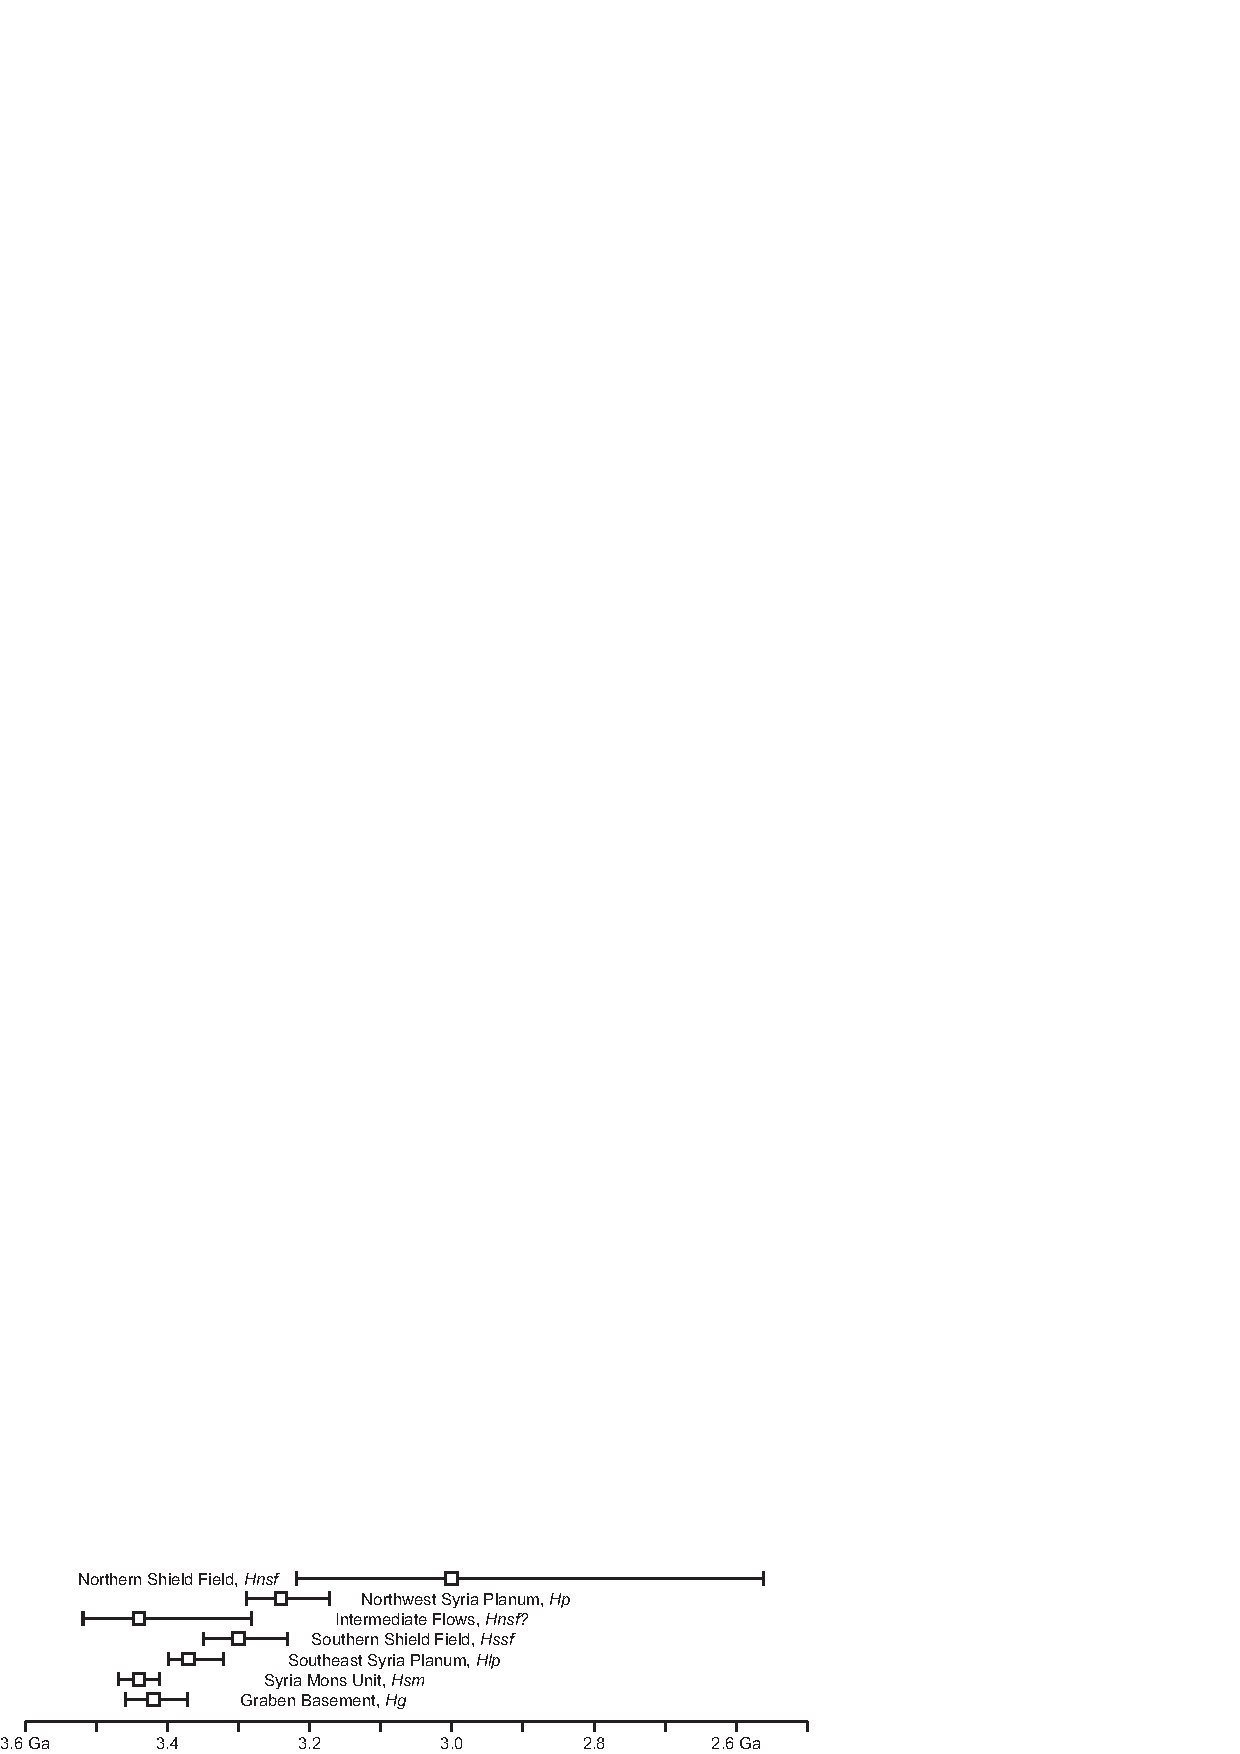
\includegraphics[width=178mm]{../fig2.png}
\caption{2011-2013 velocity maps obtained using TRI (left) and TerraSAR-X (right). Both TRI and TerraSAR-X velocities were adjusted to match the direction of ice motion (140$^{\circ}$ counterclockwise from north) using Equation 3. Note the similarity in velocity magnitude and distribution between the TRI and satellite maps despite the different acquisition and averaging times (3.5 hours for the TRI vs 11 days for TerraSAR-X).}
\label{fig:velmaps}
\end{figure*}

\begin{figure*}
\centering
\includegraphics[width=178mm]{erf.png}
\caption{Differences between the TerraSAR-X and TRI velocity maps in the direction of ice motion. Despite different sampling periods (11 days vs 3.5 hours), the agreement between the TRI and TerraSAR-X is reasonable (rms difference of  \textasciitilde1~m/d for all years) except for areas near crevasses and a small region near the highly-dynamic terminal zone.}
\label{fig:velmapserror}
\end{figure*}



% \pagebreak
\begin{figure*}
\centering
\includegraphics[width=178mm]{combofig.png}
\caption{
Terminus outlines from TRI and LANDSAT for the period 2008-2013, and the location of points discussed in the paper. Displacement (v) and noise (n) time series points from 2011 and 2012 are shown along with the BSOP/CTD locations. Points v1, v2, and v3 are velocity measurements from 2012 located on the moving ice. Points n1, n2, and n3 are stationary areas used to assess noise characteristics in 2012. Point n1 is located on moraine
deposits near the lagoon shore. Point n2 is located on a mountain. Point n3 is located on
stagnant ice near a medial moraine. Points 1, 2, and 3 show the locations on the ice selected for tidal comparisons in 2011. The marked lines show the terminus positions and embayment dynamics observed by LANDSAT and TRI. Note that the embayment opens during the summer of 2012 and 2013, and partially closes during the winter/spring of 2013 and 2014. }
\label{fig:12tslocs}
\label{fig:11tidelocs}
\label{fig:retreat}
\end{figure*}

% \pagebreak
\begin{figure*}                  
\centering
\includegraphics[width=178mm]{new_figures/vel12.pdf}       
\caption{Displacement time series, 2012, for the points shown in Figure \ref{fig:12tslocs}. A (top) shows actual displacement, B (bottom) shows detrended displacement. Labels in the top panel show the location, the distance from the radar, the best-fit velocity, and the rms uncertainty for the three points on the glacier. Variations in velocity and rms scatter are related to distance from the glacier terminus (velocity and rms scatter decrease with increasing distance)}
\label{fig:ts12}
\end{figure*}

% \pagebreak
\begin{figure*}         
\centering
\includegraphics[width=178mm]{new_figures/nz12.pdf}       
\caption{Similar to Figure \ref{fig:ts12}, displacement time series, 2012, for stationary targets (a measure of noise). Location of points shown in Figure \ref{fig:12tslocs}. A (top) shows the actual displacement. B (bottom) shows the detrended displacement. Labels in the top panel show the point location, distance from the radar, linear velocity, and rms displacement from zero.}
\label{fig:nzts12}
\end{figure*}

% % \pagebreak
% \begin{figure} 
% \centering 
% \includegraphics[trim= .2cm .2cm .2cm .2cm, clip=true,width=86mm]{new_figures/2011tidelocs.pdf}
% \caption{Locations on the ice selected for tidal comparisons, 2011.}
% \label{fig:11tidelocs}
% \end{figure}



% \pagebreak
\begin{figure*}
\centering
\includegraphics[width=178mm]{new_figures/avgnz.pdf}
\caption{A comparison of theoretical rate error (Equation 7) to line-of-sight velocity uncertainties for different averaging times for the stationary points shown in Figure \ref{fig:12tslocs}.}
\label{fig:12error}
\end{figure*}

% \pagebreak
\begin{figure*}               
\centering
\includegraphics[width=178mm]{new_figures/tide11.pdf}        
\caption{Displacement and tide time series, 2011. Top panel shows total displacement for three points (Figure \ref{fig:12tslocs}) and tides (black line). Bottom panel shows detrended displacement and tides. Small calving events can be seen in the tidal record. There are no apparent velocity variations associated with the tidal signal over the short acquisition period, but longer time series are necessary for a more thorough analysis.}
\label{fig:11tidedisp}
\end{figure*}





% % \pagebreak
% \begin{figure}
% \centering
% %\includegraphics[trim= .2cm .2cm .2cm .2cm, clip=true, width=86mm]{new_figures/retr.pdf}
% \includegraphics[trim= .2cm .2cm .2cm .2cm, clip=true, width=86mm]{termmap.pdf}
% \caption{Terminus retreat and embayment dynamics observed by LANDSAT and TRI. Note the formation, closing, and reappearance
% of the embayment in 2008, 2012, and 2013.}
% \label{fig:retreat}
% \end{figure}

% \pagebreak
\begin{figure*}
\centering
\includegraphics[width=178mm]{new_figures/demoutputnew.png}
\caption{A perspective view of the smoothed TRI-derived DEMs in 2011 and 2012, and their difference. There is substantial ice loss immediately adjacent to the terminus.}\label{fig:dems}
\label{fig:demperspective}
\end{figure*}






% \pagebreak
\begin{figure*}
\centering
\includegraphics[width=178mm]{lossmapnew.png}
\caption{Map of ice loss between 2011 and 2012. Note that most of the ice was lost in the region around the seasonal embayment. The colored boxes show the areas used for ASTER/TRI DEM comparsions (yellow) and the 2011-2012 TRI DEM comparisons (cyan).}
\label{fig:dems}
\end{figure*} 


\begin{figure*}
\centering
\includegraphics[width=178mm]{new_figures/vel_elev_annotated.png}
\caption{Smoothed line-of-sight velocity and elevation profiles in the vicinity of the terminus along the center line of the imaged area in 2011 and 2012. The inset at the top left shows the approximate surface slopes near and upglacier of the ice cliff.}
\label{fig:velelev}
\end{figure*}


\begin{figure*}
\centering
\includegraphics[width=178mm]{new_figures/eis.png}
\caption{Counterclockwise iceberg motion through the embayment in 2012. This kind of circulation may represent horizontally partitioned flow, where surface and near surface lagoon waters flow into the embayment and circulate in a counterclockwise direction with fast velocities. Here, he iceberg enters the embayment at a speed of \textasciitilde6 cm/s, accelerates to \textasciitilde18 cm/s as it passes through, and slows down to \textasciitilde7~cm/s as it exits the embayment on the other side into the open water. This suggests that there may be high fluxes of water passing through the embayment.}
\label{fig:icemotion}
\end{figure*}


\begin{figure*}
\centering
\includegraphics[width=178mm]{new_figures/outflow.png}
\caption{A five-hour period showing an outflow event observed in 2012. Such outflow events may represent vertically partitioned flows where cold, fresh meltwater emerges from the base of a glacier, rapidly rises to the surface and flows outward as a broad, shallow surface current pushing out  the nearby icebergs. The iceberg closest to the center of the lagoon (cyan) gets pushed away from the vicinity of the terminus. Note the slower speed and the clockwise trend shown by the icebergs (circled in red and yellow) that are less affected by the outflow event.}
\label{fig:OFQ}
\end{figure*}


% \pagebreak
\begin{figure*}
\centering
\includegraphics[width=178mm]{2yrs.pdf}
\caption{Lagoon salinity and temperature profiles from the 2012 BSOP deployment and the 2013 CTD casts showing that  Jökulsárlón is well-mixed with only slightly warmer, saltier 
water at the bottom. The data consist of multiple casts (to various depths) for each instrument. The cast locations are shown in Figure \ref{fig:retreat}, and illustrate some of the depth variability within the lagoon. The CTD locations were closer to the deeper central portion of the lagoon, while the BSOP locations were closer to shore. Small outlying points may be related to the CTD hitting the lagoon bottom.}
\label{fig:ctd}
\end{figure*}


\begin{figure*}
\centering
%\includegraphics[width=86mm]{new_figures/mixplots.pdf}
\includegraphics[width=178mm]{ctdfig.png}
\caption{BSOP and CTD data showing the mixed properties of the lagoon water in comparsion to two linear mixing models. The two endmember waters appear to be a 0$^{\circ}$C, 0 psu salinity freshwater and an ocean water with temperature between 4 and 6$^{\circ}$C and salinity 35 psu (warmer temperatures in the upper left reflect atmospheric warming in the top 5 meters). A Gade line with a typical slope of 2.5$^{\circ}$C/psu is shown, suggesting that late-summer measurements are not significantly affected by ocean-forced melting. Outliers below a salinity of 1 were discarded.}
\label{fig:mplots}
\end{figure*}






\end{document}
